\documentclass[11pt]{article}
\usepackage[margin=1in]{geometry}
\usepackage[T1]{fontenc}
\usepackage[sc]{mathpazo}
\linespread{1.05}
\usepackage{microtype}
\usepackage{amsmath,amssymb,amsthm}
\usepackage{booktabs}
\usepackage{graphicx}
\usepackage{caption}
\usepackage{xcolor}
\usepackage[authoryear,round]{natbib}
\usepackage[colorlinks=true,linkcolor=blue!50!black,citecolor=blue!50!black,urlcolor=blue!50!black]{hyperref}

% generated by build_assets.py -- do not edit
\newcommand{\NRaw}{4,092}
\newcommand{\NCrossed}{20}
\newcommand{\NZeroBid}{408}
\newcommand{\NWide}{16}
\newcommand{\NIV}{1,624}
\newcommand{\IVErrMed}{1.2}
\newcommand{\IVErrPnf}{9.8}
\newcommand{\FwdErrMax}{0.37}
\newcommand{\RImpMin}{1.47}
\newcommand{\RImpMax}{4.62}
\newcommand{\SVIRmseMax}{21.5}
\newcommand{\SVIgMin}{0.27}
\newcommand{\SVILeeMax}{0.120}
\newcommand{\CalMinGap}{2.5}
\newcommand{\VIXRep}{16.541}
\newcommand{\VIXTrue}{16.543}
\newcommand{\VIXErr}{\ensuremath{-}0.0017}
\newcommand{\VIXErrAbs}{0.002}
\newcommand{\VIXInterp}{16.546}
\newcommand{\VIXSVI}{16.550}
\newcommand{\NearN}{242}
\newcommand{\NextN}{271}
\newcommand{\CalVzero}{0.0262}
\newcommand{\CalKappa}{2.1042}
\newcommand{\CalTheta}{0.0405}
\newcommand{\CalSigma}{0.7801}
\newcommand{\CalRho}{\ensuremath{-}0.7103}
\newcommand{\CalRmse}{2.3}
\newcommand{\CalSec}{1.9}
\newcommand{\CalNfev}{25}
\newcommand{\Feller}{\ensuremath{-}0.44}
\newcommand{\MCWithin}{94}
\newcommand{\MCMaxZ}{2.79}
\newcommand{\MCSec}{7.9}
\newcommand{\MCAbsErr}{0.46}
\newcommand{\ASeeds}{200}
\newcommand{\AInterp}{+0.0033}
\newcommand{\ATruncFive}{\ensuremath{-}0.0064}
\newcommand{\ATruncHundred}{\ensuremath{-}0.0084}
\newcommand{\ADiscFive}{+0.0004}
\newcommand{\ADiscTwentyFive}{+0.0087}
\newcommand{\ADiscFifty}{+0.0337}
\newcommand{\ADiscHundred}{+0.136}
\newcommand{\ADiscHundredAbs}{0.14}
\newcommand{\ANoiseSdFive}{0.0010}
\newcommand{\ANoiseSdHundred}{0.0040}
\newcommand{\ATotalFive}{\ensuremath{-}0.0025}
\newcommand{\ATotalHundred}{+0.130}
\newcommand{\AThetaCoef}{1.30}
\newcommand{\AEmpCoef}{1.36}
\newcommand{\FPCMin}{1.012}
\newcommand{\FPCMax}{1.039}
\newcommand{\IdentityRel}{2\times 10^{-6}}
\newcommand{\BSeeds}{40}
\newcommand{\BKappaSdFull}{0.4}
\newcommand{\BKappaSdShort}{6.1}
\newcommand{\BThetaSdFull}{0.2}
\newcommand{\BThetaSdShort}{3.2}
\newcommand{\BRhoSdShort}{0.2}
\newcommand{\BSigmaSdShort}{0.4}
\newcommand{\BCorrKTShort}{\ensuremath{-}0.95}
\newcommand{\BCorrKTFull}{\ensuremath{-}0.69}
\newcommand{\BRatioMinFull}{1.4}
\newcommand{\BRatioMaxFull}{2.4}
\newcommand{\BRatioMaxShort}{3.1}
\newcommand{\BRatioThetaFull}{2.25}
\newcommand{\BRatioThetaTF}{1.19}
\newcommand{\BRatioVzeroFull}{1.83}
\newcommand{\BRatioVzeroTF}{1.20}
\newcommand{\BRatioSigmaTF}{1.68}
\newcommand{\BRatioRhoTF}{2.05}
\newcommand{\BThetaSdTF}{0.11}
\newcommand{\BThetaSdFullP}{0.21}
\newcommand{\BKappaMADShort}{4.4}
\newcommand{\BThetaMADShort}{1.6}
\newcommand{\BKappaMADFull}{0.4}
\newcommand{\BThetaMADFull}{0.2}
\newcommand{\OSeed}{23}
\newcommand{\ORmse}{5.2}
\newcommand{\ORmseMed}{2.7}
\newcommand{\OKappa}{1.49}
\newcommand{\OTheta}{0.0474}
\newcommand{\OStrike}{6325}
\newcommand{\OBid}{0.10}
\newcommand{\OAsk}{0.25}
\newcommand{\OTrue}{0.23}
\newcommand{\OMidErr}{\ensuremath{-}62}
\newcommand{\OResid}{54}
\newcommand{\ODropKappa}{1.95}
\newcommand{\ORobKappa}{1.87}
\newcommand{\MCMartMax}{3.1\times 10^{-4}}
\newcommand{\MCMartZ}{0.8}
\newcommand{\MCMartDays}{308}
\newcommand{\RSVIGap}{0.001}
\newcommand{\RHestonSpread}{2\times 10^{-6}}
\newcommand{\RMCSeedMax}{1.34}
\newcommand{\RMCDaily}{1.16}
\newcommand{\RMCWeekly}{0.65}


\newtheorem{proposition}{Proposition}
\theoremstyle{remark}
\newtheorem*{remark}{Remark}
\captionsetup{font=small,labelfont=bf}
\newcommand{\dK}{\Delta K}

\title{\textbf{How Accurate Is a Volatility-Surface Pipeline?}\\[2pt]
\large A Ground-Truth Study of SVI Fitting, VIX Replication and Heston Calibration on SPX Options}
\author{Kaiki Ikeda}
\date{February 2026}

\begin{document}
\maketitle

\begin{abstract}
\noindent
We build an end-to-end pipeline for the SPX implied-volatility surface and evaluate it in a setting where the right answer is known.
Option quotes for a nominal close on 13~February~2026 are simulated from a Heston model and then degraded the way a raw vendor snapshot is: bid--ask spreads, tick rounding, zero bids in the wings and a small share of erroneous quotes.
Against this ground truth we report three findings.
First, raw SVI slices fitted to each expiry are free of static arbitrage, but carry up to \SVIRmseMax~bp of shape error at one-to-six-month maturities that no optimiser removes; the error vanishes at the long end, consistent with SVI being the large-maturity limit of Heston.
Second, Cboe's VIX methodology recovers the true 30-day variance-swap volatility to within \VIXErrAbs{} vol points.
Decomposing the error, we show analytically and numerically that on a uniform strike grid the discretisation bias is $\dK^2/(6TF^2)$ in variance, independent of where the forward falls between strikes: negligible at 5-point spacing, but \ADiscHundredAbs{} vol points at 100.
Third, Heston parameters are recovered to better than 0.5\% from the full surface, but mean reversion and long-run variance are weakly identified from expiries of 35 days or less (correlation \BCorrKTShort), a single cheap wing quote can move the mean-reversion estimate from \ODropKappa{} to \OKappa, and Gauss--Newton standard errors understate the dispersion across noise draws by a factor of \BRatioMinFull--\BRatioMaxShort.
All data are simulated; code, data and a C++ Monte Carlo pricer are released with the paper.
\end{abstract}

\section{Introduction}

Every desk that trades index options maintains some version of the same pipeline: clean a chain of quotes, back out implied volatilities, fit a smooth arbitrage-free surface, compute model-free quantities such as the VIX, and calibrate a stochastic-volatility model for pricing and risk.
Each stage introduces error, but with market data the size of that error is hard to measure, because the true surface is never observed.
A fit that matches quotes closely may still be systematically wrong; a replicated VIX that differs from the published index may reflect a bug, a methodological choice, or genuine noise.

This paper takes the opposite approach: it runs the full pipeline on quotes generated from a known model, so that every intermediate quantity has a ground truth to be graded against.
The data-generating model is Heston \citep{heston1993}, calibrated to plausible SPX levels for mid-February 2026 (spot 6{,}836, ATM implied volatility around 15--16\%, steep negative skew).
The quotes are then degraded with a simple but realistic microstructure model.
This is a controlled experiment rather than an empirical study; we return to what it can and cannot show in Section~\ref{sec:limits}.

The design lets us separate questions that are usually entangled:
\begin{enumerate}
  \item \textbf{Surface fitting.} When raw SVI \citep{gatheral2004} misses the quotes, is the problem the optimiser, the noise, or the functional form? (Section~\ref{sec:svi})
  \item \textbf{VIX replication.} How large are the truncation, discretisation, interpolation and quote-noise errors in Cboe's methodology, and how do they scale with strike spacing? (Section~\ref{sec:vix})
  \item \textbf{Model calibration.} Which Heston parameters do option quotes actually pin down, and are standard errors from a single calibration trustworthy? (Section~\ref{sec:heston})
\end{enumerate}
The main contribution beyond the validation itself is Proposition~\ref{prop:disc}: a closed-form leading-order expression for the discretisation bias of the Cboe estimator, together with the observation that the estimator's at-the-money adjustments exactly remove any dependence on the forward's position between strikes.

\section{Related literature}

The replication of variance by a static portfolio of options goes back to \citet{breedenlitzenberger1978}, who showed that the second strike derivative of call prices recovers the risk-neutral density, and was developed into a theory of variance trading by \citet{carrmadan1998} and \citet{demeterfi1999}.
The VIX applies this result to listed SPX options \citep{cboevix}.
\citet{jiangtian2005} study model-free implied volatility in general, and \citet{jiangtian2007} examine the VIX calculation specifically, documenting truncation and discretisation errors numerically.
\citet{carrwu2009} discuss the approximation error of the replication when the underlying can jump.
Our decomposition in Section~\ref{sec:vix} complements this work with an exact ground truth and an analytic expression for the discretisation term.

For the surface, SVI was introduced by \citet{gatheral2004} and is discussed at length in \citet{gatheral2006}.
\citet{gatheraljacquier2011} show that SVI is the large-maturity limit of the Heston smile, and \citet{gatheraljacquier2014} derive the no-butterfly-arbitrage condition we test and propose the SSVI extension.
\citet{lee2004} bounds the asymptotic slope of total implied variance.
\citet{demarcomartini2009} give the quasi-explicit calibration we use as a robustness check.

For Heston pricing we use the single-integral representation of \citet{lewis2000} with the numerically stable characteristic function of \citet{albrecher2007}; for simulation, the Quadratic-Exponential scheme of \citet{andersen2008}.

\section{Data-generating process and pipeline}
\label{sec:method}

\subsection{Snapshot and hidden model}

The snapshot is the 4:00\,pm close on Friday 13~February~2026, with spot $S_0 = 6{,}836.17$, a flat rate $r = 3.65\%$ and dividend yield $q = 1.18\%$.
These are illustrative values, not observed market data.
Nine expiries span 7 to 308 days, mixing PM-settled weeklies and AM-settled monthlies; the June monthly expires on Thursday 18 June because 19 June 2026 is a market holiday.
Time to expiry is measured in calendar minutes, as in the VIX methodology.

Prices are generated from the Heston model
\begin{equation}
  \frac{dF_t}{F_t} = \sqrt{v_t}\, dW_t, \qquad
  dv_t = \kappa(\theta - v_t)\,dt + \sigma\sqrt{v_t}\, dZ_t, \qquad
  d\langle W, Z\rangle_t = \rho\, dt,
\end{equation}
written under the $T$-forward measure, with hidden parameters
\[
  (v_0, \kappa, \theta, \sigma, \rho) = (0.0262,\ 2.10,\ 0.0405,\ 0.78,\ -0.71).
\]
These give an ATM volatility of about 16\% and violate the Feller condition ($2\kappa\theta < \sigma^2$), as calibrated SPX parameters typically do.

\subsection{Microstructure model}

For each strike the true price $P$ is turned into a quote.
The spread is
\[
  s = \min\!\big(\max(0.05 + 0.015P,\ 0.10),\ 0.08P + 0.10\big);
\]
the mid is jittered by $0.12\,s\,\varepsilon$ with $\varepsilon \sim N(0,1)$; bid and ask are rounded outward to the SPX tick (0.05 below \$3, 0.10 above); and the bid is set to zero when the option is worth less than a tick.
On top of this, 1\% of quotes are corrupted: half become crossed markets, half get a stale, inflated ask.
The resulting chain has \NRaw{} quotes.

\subsection{Pipeline}

\paragraph{Cleaning, forwards and implied volatilities.}
We drop \NCrossed{} crossed quotes, \NZeroBid{} zero bids and \NWide{} quotes whose relative spread exceeds 50\%.
For each expiry, the forward and discount factor are estimated by regressing $C - P$ on strike over near-the-money pairs, using put--call parity $C - P = D(F - K)$.
Implied volatilities are Black-76 inversions of out-of-the-money mids on the estimated forward, leaving \NIV{} quotes.

\paragraph{SVI slices.}
For each expiry, with $k = \ln(K/F)$ and total implied variance $w = \sigma_{\mathrm{imp}}^2 T$, we fit
\begin{equation}
  w(k) = a + b\left(\rho_s (k - m) + \sqrt{(k-m)^2 + s^2}\right)
\end{equation}
by weighted least squares in implied-volatility space, with weights equal to the inverse implied-volatility half-spread, twelve starting points, and the constraint $a + bs\sqrt{1-\rho_s^2} \ge 0$ that keeps $w$ non-negative.

\paragraph{Static-arbitrage checks.}
A slice is free of butterfly arbitrage if and only if the implied density is non-negative, which \citet{gatheraljacquier2014} show is equivalent to
\begin{equation}
  g(k) = \left(1 - \frac{k w'}{2w}\right)^2 - \frac{w'^2}{4}\left(\frac{1}{w} + \frac14\right) + \frac{w''}{2} \ \ge\ 0 .
\end{equation}
We evaluate $g$ on the quoted range and 0.5 beyond it in each direction.
Lee's moment formula requires the wing slopes $b(1 \pm \rho_s)$ to be at most 2.
The surface is free of calendar arbitrage if $w(k, T)$ is non-decreasing in $T$ at every $k$; we check this on a grid $k \in [-1.2, 0.5]$.

\paragraph{VIX.}
We follow the Cboe methodology literally.
The near and next terms are the expiries with more than 23 and fewer than 37 days to settlement (here 13 March, 28.0 days, and 20 March, 34.7 days).
For each term, $F$ is set from the strike with the smallest $|C - P|$, $K_0$ is the first strike at or below $F$, and strikes are included moving outward from $K_0$ until two consecutive zero bids.
The term variance is
\begin{equation}
  \hat\sigma^2 = \frac{2}{T}\sum_i \frac{\dK_i}{K_i^2} e^{RT} Q(K_i) - \frac{1}{T}\left(\frac{F}{K_0} - 1\right)^2,
  \label{eq:vix}
\end{equation}
where $Q(K_i)$ is the out-of-the-money mid (the call--put average at $K_0$), and the two terms are interpolated linearly in total variance to 30 days.
Because the data contain no jumps, the target is known exactly: the 30-day fair variance
$\mathbb{E}\big[\tfrac{1}{\tau}\int_0^\tau v_t\,dt\big] = \theta + (v_0 - \theta)\,\frac{1 - e^{-\kappa\tau}}{\kappa\tau}$.
We use a single flat rate for both terms, where Cboe interpolates Treasury yields per term.

\paragraph{Heston calibration.}
Model prices use the Lewis single-integral formula with the characteristic function of \citet{albrecher2007}, integrated by 600-node Gauss--Legendre quadrature on a maturity-dependent range; prices agree with adaptive quadrature to about $10^{-4}$ index points.
We minimise $\sum_i \big((P^{\text{model}}_i - P^{\text{mid}}_i)/\mathcal{V}_i\big)^2$, where $\mathcal{V}_i$ is Black vega, a standard proxy for implied-volatility error that avoids inverting prices at every iteration.
The calibration set is a 360-quote subsample thinned evenly across each smile, and the optimiser converges in \CalNfev{} function evaluations.

\paragraph{Monte Carlo.}
A C++ pricer simulates variance with Andersen's QE scheme and the log-forward with his central discretisation, on a time grid that lands exactly on every expiry, so that one set of paths prices the whole surface.
It runs with 200{,}000 paths at four steps per day in \MCSec{} seconds on two threads.
We use it as an independent check of the calibrated semi-analytic prices rather than inside the calibration.

\section{Implied volatilities and forwards}

Implied volatilities from cleaned mids differ from the noiseless values by a median of \IVErrMed~bp (95th percentile \IVErrPnf~bp), with the largest errors in the far wings where vega is small.

The parity regression illustrates a point that matters in practice.
The forward is tightly identified: on every expiry it lies within \FwdErrMax{} index points of the truth.
The discount factor is not: the implied rate ranges from \RImpMin\% to \RImpMax\% around the true 3.65\%.
Over a strike window of a few percent, $C - P$ is nearly linear in $K$ with a slope close to $-1$, and a small error in the slope maps into a large error in the implied rate, particularly at short maturities.
In production it is preferable to take the discount factor from the SOFR curve and estimate only the forward.

\section{SVI slices and static arbitrage}
\label{sec:svi}

\begin{figure}[t]
  \centering
  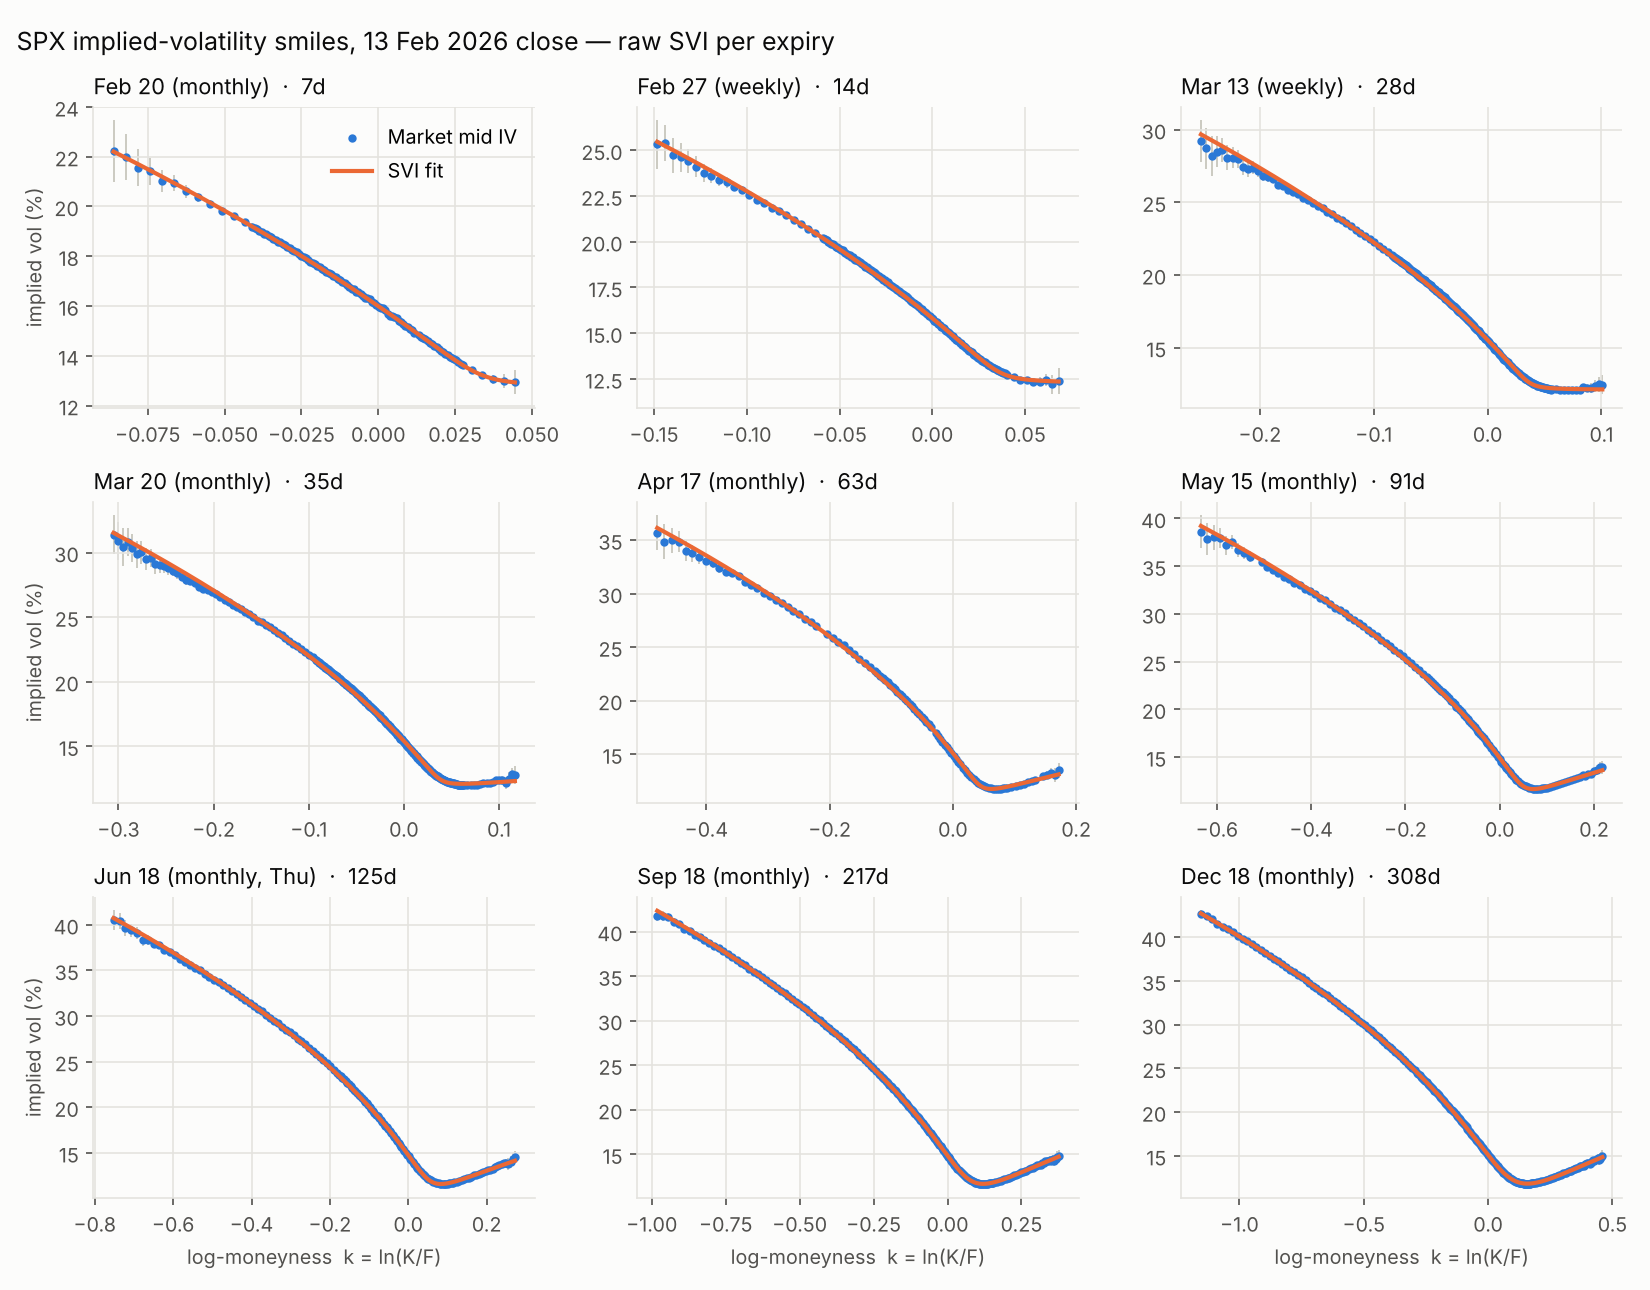
\includegraphics[width=\textwidth]{figures/fig_smiles.png}
  \caption{Market mid implied volatilities (dots, with half-spread bars) and fitted raw SVI slices for the nine expiries.}
  \label{fig:smiles}
\end{figure}

\begin{table}[t]
  \centering\small
  \begin{tabular}{lrrrrrr}
\toprule
Expiry & $n$ & RMSE & RMSE & in & $\min g$ & Lee \\
 & & quotes (bp) & truth (bp) & spread & & slope \\
\midrule
Feb 20 (7d) & 110 & 3.3 & 3.9 & 100\% & 0.32 & 0.005 \\
Feb 27w (14d) & 166 & 7.4 & 8.5 & 93\% & 0.31 & 0.010 \\
Mar 13w (28d) & 242 & 15.8 & 14.2 & 52\% & 0.30 & 0.020 \\
Mar 20 (35d) & 271 & 16.1 & 16.6 & 45\% & 0.30 & 0.024 \\
Apr 17 (63d) & 105 & 21.5 & 20.9 & 42\% & 0.29 & 0.039 \\
May 15 (91d) & 132 & 18.7 & 17.9 & 46\% & 0.28 & 0.052 \\
Jun 18 (125d) & 157 & 12.9 & 13.2 & 54\% & 0.28 & 0.066 \\
Sep 18 (217d) & 202 & 6.2 & 4.1 & 99\% & 0.27 & 0.097 \\
Dec 18 (308d) & 239 & 3.4 & 1.7 & 100\% & 0.27 & 0.120 \\
\bottomrule
\end{tabular}

  \caption{SVI fit by expiry. ``RMSE truth'' compares the fit with the noiseless implied volatilities. ``In spread'' is the share of strikes where the fit lies inside the implied-volatility half-spread. $\min g$ is the minimum of Gatheral's butterfly function over the quoted range extended by 0.5 in log-moneyness. Lee slope is $\max b(1\pm\rho_s)$; the bound is 2.}
  \label{tab:svi}
\end{table}

Figure~\ref{fig:smiles} and Table~\ref{tab:svi} summarise the fits.
All nine slices pass every static-arbitrage test.
The minimum of $g$ is \SVIgMin, so the implied densities are strictly positive.
The largest wing slope, \SVILeeMax, is far below Lee's bound.
Total variance increases with maturity at every log-moneyness, with a smallest gap of $\CalMinGap \times 10^{-4}$ between the 13 March and 20 March slices (Figure~\ref{fig:arb}).

\begin{figure}[t]
  \centering
  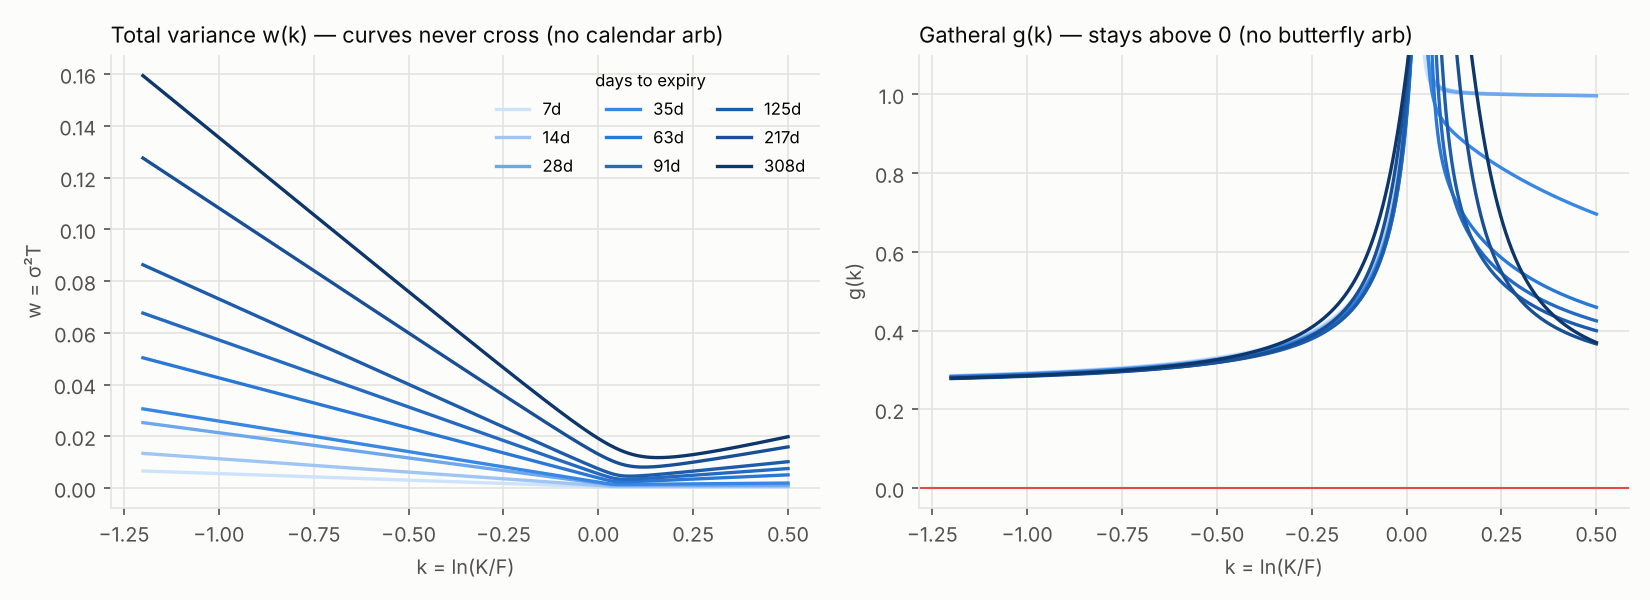
\includegraphics[width=\textwidth]{figures/fig_arbitrage.png}
  \caption{Left: total implied variance by expiry; the curves never cross, so there is no calendar arbitrage. Right: Gatheral's $g(k)$, which stays strictly positive, so there is no butterfly arbitrage.}
  \label{fig:arb}
\end{figure}

The fit quality, however, is uneven.
At 7 and 308 days SVI sits inside the bid--ask spread almost everywhere.
Between one and six months the RMSE rises to \SVIRmseMax~bp and only around half of the fitted values lie inside the spread.
Two pieces of evidence show that this is a limitation of the functional form rather than of the fitting procedure.
First, the quasi-explicit method of \citet{demarcomartini2009}, which solves for three of the five parameters in closed form and searches only over the remaining two, produces curves within \RSVIGap~bp of the multi-start fit on every slice.
Second, the error against the \emph{noiseless} implied volatilities is as large as the error against the quotes (Table~\ref{tab:svi}); noise in the quotes is not what the fit is missing.

Figure~\ref{fig:svierr} shows the shape of the residual.
The misfit is structured: SVI overshoots in the deep put wing and oscillates around the money.
This is consistent with \citet{gatheraljacquier2011}, who show that SVI is exact for Heston only as maturity tends to infinity; at the 308-day expiry the error has nearly vanished.
At 7 to 14 days the quoted range spans too little log-moneyness for the shape difference to show.
The practical consequence is that adding optimiser restarts would not help; a richer parameterisation such as SSVI \citep{gatheraljacquier2014} is the natural next step.

\begin{figure}[t]
  \centering
  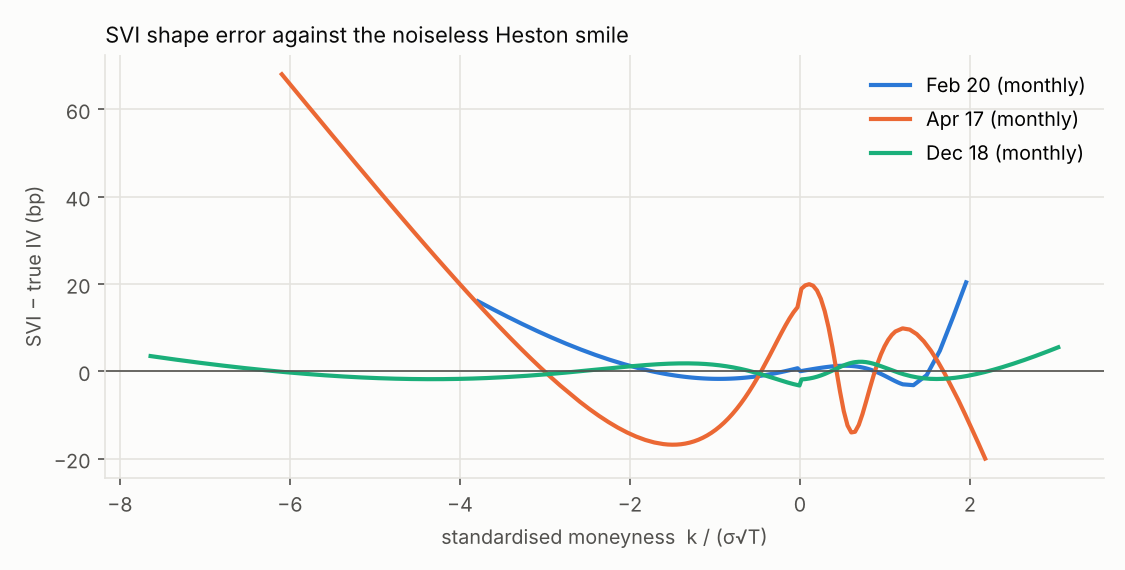
\includegraphics[width=0.75\textwidth]{figures/fig_svi_error.png}
  \caption{SVI minus noiseless implied volatility, against standardised moneyness, for three expiries. The structured error at 63 days is a property of the functional form.}
  \label{fig:svierr}
\end{figure}

\section{VIX replication}
\label{sec:vix}

\subsection{Baseline}

On the generated chain, the replicated VIX is \VIXRep{} against a true 30-day value of \VIXTrue, an error of \VIXErr{} vol points.
The near and next terms use \NearN{} and \NextN{} strikes.
Two benchmarks help interpret this.
Interpolating the \emph{exact} term variances to 30 days gives \VIXInterp, so linear interpolation in total variance alone accounts for a bias of \AInterp.
Integrating the fitted SVI smiles over a continuum of strikes, with no truncation or discretisation, gives \VIXSVI; the gap to the truth there reflects SVI's shape error rather than the replication formula.
Figure~\ref{fig:vixcontrib} shows where the variance comes from: the integrand peaks at the money and decays quickly, more slowly on the put side.

\begin{figure}[t]
  \centering
  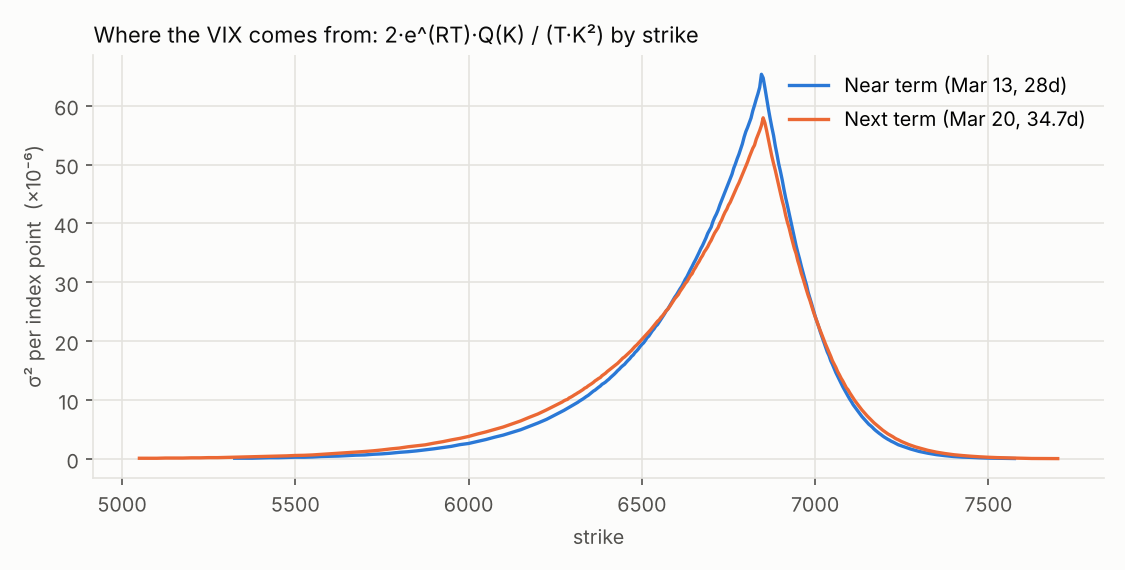
\includegraphics[width=0.75\textwidth]{figures/fig_vix.png}
  \caption{Per-index-point contribution to term variance, $2e^{RT}Q(K)/(TK^2)$, for the near and next VIX terms.}
  \label{fig:vixcontrib}
\end{figure}

\subsection{Error decomposition across strike spacings}

To study how the error depends on the strike grid, we re-run the near and next terms on uniform grids with spacing $\dK \in \{5, 10, 25, 50, 100\}$ and decompose the error sequentially:
\begin{enumerate}
  \item \emph{interpolation}: the exact term variances, interpolated to 30 days, versus the exact 30-day value;
  \item \emph{truncation}: a continuum integral of true prices over the strike range kept by the two-zero-bid rule, versus the full integral;
  \item \emph{discretisation}: Equation~\eqref{eq:vix} on that range with true mid prices, versus the continuum integral;
  \item \emph{quote noise}: Equation~\eqref{eq:vix} on dressed quotes, averaged over \ASeeds{} independent noise draws.
\end{enumerate}
As a sanity check on the target itself, the continuum integral over a very wide range reproduces the exact term variances to a relative error of $\IdentityRel$, confirming the replication identity for this diffusion.

\begin{table}[t]
  \centering\small
  \begin{tabular}{rrrrrrr}
\toprule
$\Delta K$ & strikes & interp. & trunc. & discret. & quote noise & total \\
 & near/next & & & & mean $\pm$ s.d. & mean \\
\midrule
5 & 460/532 & +0.0033 & \ensuremath{-}0.0064 & +0.0004 & $+0.0001 \pm 0.0010$ & \ensuremath{-}0.0025 \\
10 & 230/266 & +0.0033 & \ensuremath{-}0.0065 & +0.0015 & $+0.0005 \pm 0.0014$ & \ensuremath{-}0.0012 \\
25 & 92/107 & +0.0033 & \ensuremath{-}0.0066 & +0.0087 & $+0.0005 \pm 0.0022$ & +0.0058 \\
50 & 46/54 & +0.0033 & \ensuremath{-}0.0070 & +0.0337 & $+0.0002 \pm 0.0031$ & +0.0302 \\
100 & 23/27 & +0.0033 & \ensuremath{-}0.0084 & +0.1356 & $-0.0006 \pm 0.0040$ & +0.1299 \\
\bottomrule
\end{tabular}

  \caption{Sequential decomposition of VIX replication error, in vol points, for uniform strike grids. Quote noise is the mean and standard deviation over \ASeeds{} draws relative to the discretised value.}
  \label{tab:vixdec}
\end{table}

\begin{figure}[t]
  \centering
  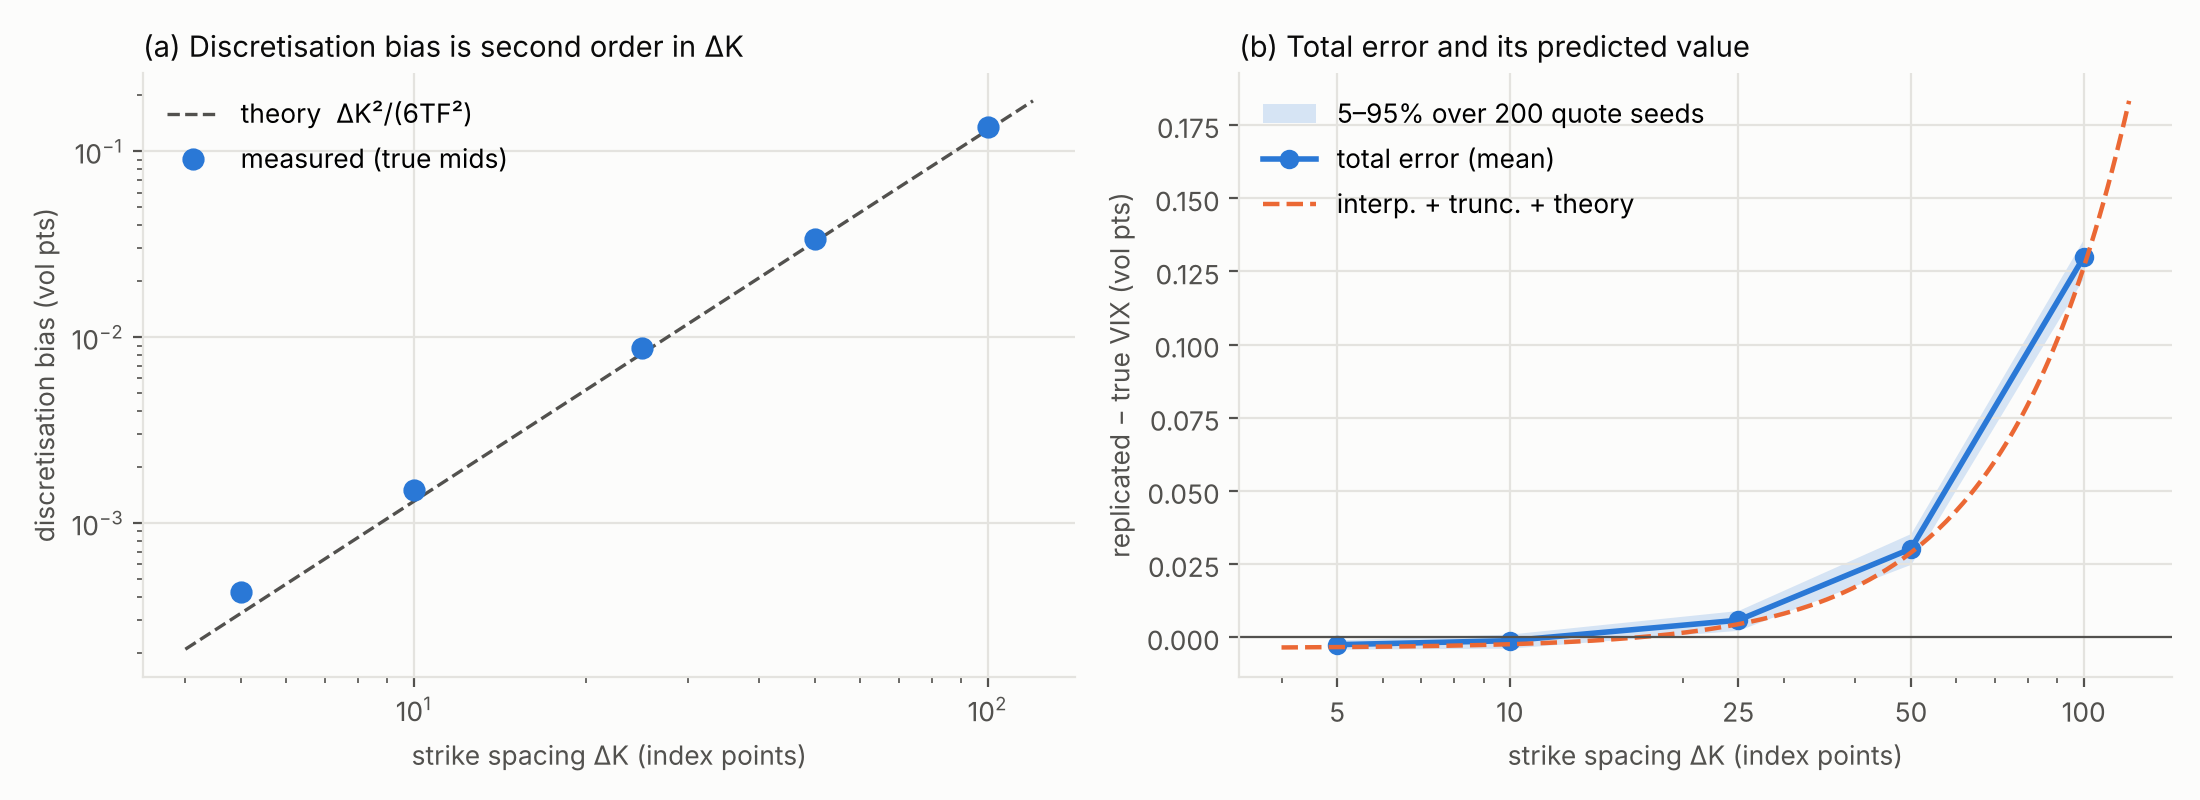
\includegraphics[width=\textwidth]{figures/fig_exp_vix.png}
  \caption{(a) Discretisation bias against strike spacing on log--log axes, with the prediction of Proposition~\ref{prop:disc}. (b) Total replication error: mean and 5--95\% band over \ASeeds{} quote-noise draws, with the sum of the interpolation, average truncation and predicted discretisation terms.}
  \label{fig:expvix}
\end{figure}

Table~\ref{tab:vixdec} and Figure~\ref{fig:expvix} give the results.
The interpolation bias is fixed at \AInterp.
Truncation contributes between \ATruncFive{} and \ATruncHundred: the two-zero-bid rule discards the far wings, and coarser grids reach the zero-bid region slightly sooner.
Quote noise is unbiased and small, with a standard deviation of \ANoiseSdFive{} vol points at 5-point spacing and \ANoiseSdHundred{} at 100, because errors on individual quotes average out across hundreds of strikes.

Discretisation dominates at coarse spacings: \ADiscFive{} at $\dK=5$, \ADiscTwentyFive{} at 25, \ADiscFifty{} at 50 and \ADiscHundred{} at 100.
The bias quadruples each time the spacing doubles.
The following result explains the scaling and predicts the constant.

\begin{proposition}
\label{prop:disc}
Let strikes lie on a uniform grid with spacing $\dK$, and write $u = (F - K_0)/\dK \in [0,1)$ for the position of the forward between strikes.
Suppose the option prices are those of a model with a smooth risk-neutral density, and that the strike range is wide enough for boundary terms to be negligible.
Then the estimator~\eqref{eq:vix} satisfies
\begin{equation}
  \hat\sigma^2 - \sigma^2_{\text{cont}} = \frac{\dK^2}{6\,T F^2} + O(\dK^3),
\end{equation}
where $\sigma^2_{\text{cont}}$ is the continuum replication integral over the same range.
The leading term does not depend on $u$.
\end{proposition}

\begin{proof}[Proof sketch]
Let $g(K)$ be $e^{RT}$ times the out-of-the-money price relative to $F$, and $f = g/K^2$, so that $\sigma^2_{\text{cont}} = (2/T)\int f\,dK$.
The function $f$ is smooth except at $F$, where the slope of $g$ jumps from $\mathbb{P}(S_T < F)$ to $-\mathbb{P}(S_T > F)$, so $f'$ jumps by $J = -1/F^2$.
Apply the composite trapezoidal rule.
On the two smooth pieces ending at $K_0$ and $K_0 + \dK$, the Euler--Maclaurin formula gives an error of $\tfrac{\dK^2}{12}\left[f'(F^-) - f'(F^+)\right] = \tfrac{\dK^2}{12F^2}$ to leading order.
On the cell containing the kink, the trapezoid rule applied to a function with slope jump $J$ has error (rule minus integral) $J\dK^2 u(1-u)/2 = -\dK^2 u(1-u)/(2F^2)$; the kink is concave, so the rule understates the integral there.
The estimator differs from the trapezoidal rule in two places.
At $K_0$ it uses the call--put average, which exceeds the put price by $e^{-RT}(F - K_0)/2$, adding $(2/T)\,\dK (F - K_0)/(2K_0^2) \approx u\dK^2/(TF^2)$.
It also subtracts $(F/K_0 - 1)^2/T \approx u^2 \dK^2/(TF^2)$.
Summing,
\begin{equation*}
  \hat\sigma^2 - \sigma^2_{\text{cont}} \approx \frac{\dK^2}{TF^2}\left[\frac16 - u(1-u) + u - u^2\right] = \frac{\dK^2}{6TF^2}. \qedhere
\end{equation*}
\end{proof}

\begin{remark}
The cancellation of $u$ is a property of the Cboe convention: the call--put average at $K_0$ and the correction term $(F/K_0-1)^2$ together undo the kink error wherever the forward falls.
Dropping either adjustment reintroduces the dependence: without the average the bracket becomes $\tfrac16 - u$, and without the correction it becomes $\tfrac16 + u^2$.
Because the bias is positive, a coarse strike grid makes the replicated VIX too high.
\end{remark}

For the near and next terms here, the proposition implies a bias of $\AThetaCoef \times 10^{-5}\,\dK^2$ vol points; the measured coefficient at $\dK = 100$ is $\AEmpCoef \times 10^{-5}$ (Figure~\ref{fig:expvix}a).
To test the independence from $u$ directly, we shift the grid so that the forward sits at fifteen positions across three spacings; the ratio of measured to predicted bias stays between \FPCMin{} and \FPCMax.
The remaining 1--4\% is the next-order term from curvature of the integrand within the kink cell.

For the official index, SPX lists 5-point strikes around the money in the relevant expiries, so the discretisation term is around $4 \times 10^{-4}$ vol points and the replication error is dominated by truncation and interpolation.
Our grids are uniform, whereas listed strikes are wider in the wings; since the leading term comes from the kink at the money, the near-the-money spacing should matter most, but we have not analysed non-uniform grids formally.

\section{Heston calibration and Monte Carlo}
\label{sec:heston}

\subsection{Baseline calibration}

On the main chain the calibrated parameters are
\[
  (v_0, \kappa, \theta, \sigma, \rho) = (\CalVzero,\ \CalKappa,\ \CalTheta,\ \CalSigma,\ \CalRho)
\]
against the hidden $(0.0262,\ 2.10,\ 0.0405,\ 0.78,\ -0.71)$, with an implied-volatility RMSE of \CalRmse~bp.
Three very different starting points converge to the same solution, with parameters agreeing to a relative $\RHestonSpread$, in about two seconds.
The left panel of Figure~\ref{fig:heston} shows the residuals: they are centred on zero and widen in the wings, as quote noise does.

\begin{figure}[t]
  \centering
  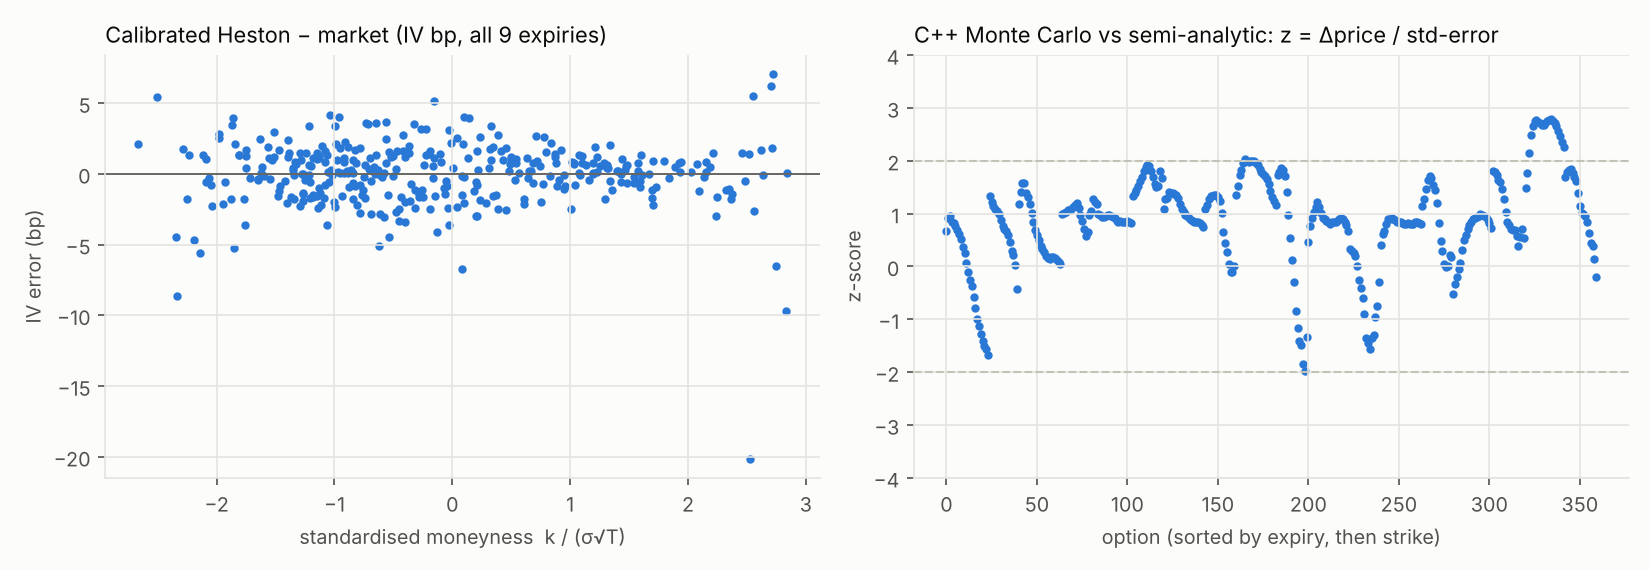
\includegraphics[width=\textwidth]{figures/fig_heston.png}
  \caption{Left: calibrated Heston minus market implied volatility. Right: Monte Carlo minus semi-analytic price, in units of the Monte Carlo standard error, for the 360 calibration options sorted by expiry and strike.}
  \label{fig:heston}
\end{figure}

Recovering the parameters of the model that generated the data is a test of the pricer and the optimiser, not of Heston as a model of SPX.
It is the minimum a calibration routine must pass, and the more informative questions are how precisely the parameters are pinned down and how reliable the reported uncertainty is.

\subsection{Identification across noise draws}

We regenerate the chain with \BSeeds{} independent noise seeds and recalibrate each in two ways: on all nine expiries, and on expiries of 35 days or less only.
Table~\ref{tab:calib} and Figure~\ref{fig:expcalib} summarise the results.

\begin{table}[t]
  \centering\small
  \begin{tabular}{lrrrrrrr}
\toprule
 & & \multicolumn{3}{c}{All 9 expiries} & \multicolumn{3}{c}{Expiries $\le$ 35 days} \\
\cmidrule(lr){3-5}\cmidrule(lr){6-8}
Param. & True & Median & s.d. (\%) & s.d./GN & Median & s.d. (\%) & s.d./GN \\
\midrule
$v_0$ & 0.0262 & 0.0262 & 0.04 & 1.83 & 0.0262 & 0.09 & 1.76 \\
$\kappa$ & 2.1 & 2.1004 & 0.37 & 1.43 & 2.1079 & 6.13 & 1.83 \\
$\theta$ & 0.0405 & 0.0405 & 0.21 & 2.25 & 0.0406 & 3.16 & 2.67 \\
$\sigma$ & 0.78 & 0.7800 & 0.12 & 1.76 & 0.7805 & 0.44 & 2.22 \\
$\rho$ & \ensuremath{-}0.71 & \ensuremath{-}0.7100 & 0.06 & 2.44 & \ensuremath{-}0.7101 & 0.24 & 3.08 \\
\bottomrule
\end{tabular}

  \caption{Heston estimates over \BSeeds{} quote-noise seeds. ``s.d.~(\%)'' is the standard deviation relative to the true value. ``s.d./GN'' is the ratio of the seed-to-seed standard deviation to the Gauss--Newton standard error from a single calibration.}
  \label{tab:calib}
\end{table}

\begin{figure}[t]
  \centering
  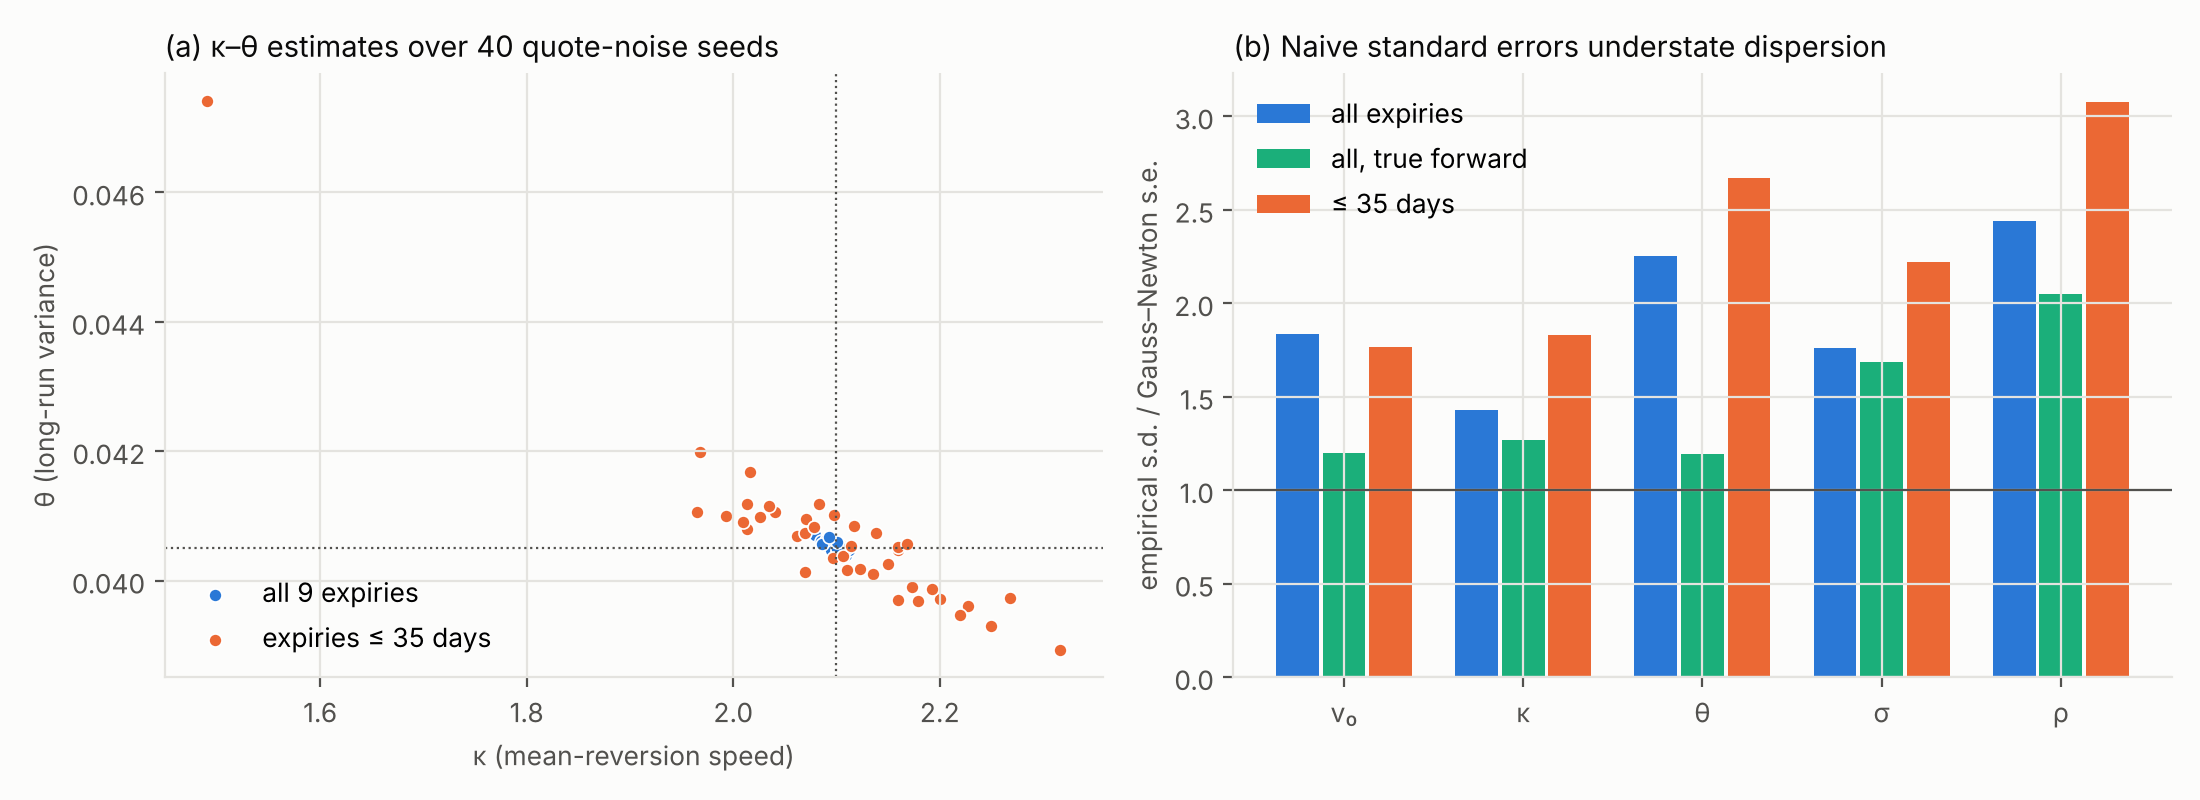
\includegraphics[width=\textwidth]{figures/fig_exp_calib.png}
  \caption{(a) Estimates of $\kappa$ and $\theta$ across seeds; dotted lines mark the true values. (b) Seed-to-seed standard deviation divided by the Gauss--Newton standard error, for the full surface, the full surface with the true forward, and short expiries only.}
  \label{fig:expcalib}
\end{figure}

\paragraph{The full surface identifies everything.}
With all expiries, every parameter has a relative standard deviation below 0.5\% and no detectable bias.

\paragraph{Short expiries do not identify mean reversion.}
With expiries of 35 days or less, $v_0$, $\sigma$ and $\rho$ remain tight (relative s.d.\ \BSigmaSdShort\% for $\sigma$ and \BRhoSdShort\% for $\rho$), but $\kappa$ and $\theta$ spread out along a ridge with correlation \BCorrKTShort{} (\BCorrKTFull{} on the full surface).
Over a month, a variance process can match the same smiles with fast reversion to a lower level or slow reversion to a higher one; only the term structure of longer expiries separates the two.
Measured robustly ($1.4826 \times$ the median absolute deviation, to discount the outlier discussed next), the spread widens from \BKappaMADFull\% to \BKappaMADShort\% for $\kappa$ and from \BThetaMADFull\% to \BThetaMADShort\% for $\theta$.

\paragraph{One quote can move the estimate.}
The most extreme short-expiry estimate, from seed \OSeed, is $\kappa = \OKappa$ and $\theta = \OTheta$, with a calibration RMSE of \ORmse~bp against a median of \ORmseMed.
Four restarts converge to the same point, so this is the optimum for that data, not a failed search.
It is driven by a single legitimate quote: a 7-day \OStrike{} put quoted \OBid/\OAsk, worth \OTrue, whose mid sits \OMidErr~bp from the truth in implied-volatility terms because the bid is pinned to the tick grid.
Dividing by its small vega gives it a residual of \OResid~bp and outsized influence.
Dropping that quote moves $\kappa$ to \ODropKappa; a soft-$L_1$ robust loss gives \ORobKappa.
Vega scaling, the standard way to approximate implied-volatility error, magnifies exactly the cheapest and least reliable quotes.
Weighting by the inverse implied-volatility spread, as we do for SVI, or using a robust loss are natural fixes.

\paragraph{Naive standard errors are too small.}
Gauss--Newton standard errors, $\hat s^2 (J^\top J)^{-1}$ from a single calibration, understate the seed-to-seed dispersion by a factor of \BRatioMinFull{} to \BRatioMaxFull{} on the full surface and up to \BRatioMaxShort{} on short expiries.
The formula assumes independent residuals, but the forward is estimated once per expiry, so its error is shared by every strike in that expiry.
Replacing the estimated forward with the true one reduces the ratio for $\theta$ from \BRatioThetaFull{} to \BRatioThetaTF{} and for $v_0$ from \BRatioVzeroFull{} to \BRatioVzeroTF{}, and halves the dispersion of $\theta$.
It leaves $\sigma$ and $\rho$ at \BRatioSigmaTF{} and \BRatioRhoTF.
A plausible remaining cause is heteroskedasticity: quote noise in implied-volatility units varies by orders of magnitude across strikes, while the formula assumes a common variance.
We have not tested this.
With \BSeeds{} seeds the ratios themselves are uncertain by roughly $\pm 0.2$.

\subsection{Monte Carlo validation}

The C++ pricer reproduces the semi-analytic prices of all 360 calibration options: \MCWithin\% lie within two Monte Carlo standard errors and all lie within three, with a largest $|z|$ of \MCMaxZ{} and a mean absolute price difference of \MCAbsErr{} index points.
Because all strikes of an expiry share paths, their errors move together (Figure~\ref{fig:heston}, right), so the effective number of independent comparisons is closer to the number of expiries.
Across seeds 1--4 the largest per-expiry mean $z$ is \RMCSeedMax; with daily and weekly time steps it is \RMCDaily{} and \RMCWeekly, so the QE scheme shows no detectable bias even at weekly steps.
The martingale check $\mathbb{E}[F_T/F_0] - 1$ is at noise level at every expiry: the largest deviation, $\MCMartMax$ at the \MCMartDays-day expiry, is \MCMartZ{} Monte Carlo standard errors.

\section{Limitations}
\label{sec:limits}

The design trades realism for a known answer, and several conclusions depend on that trade.
\begin{itemize}
  \item \textbf{Simulated data.} No quote in this paper is a market observation, and the 13 February 2026 date is nominal.
  Real chains have asynchronous quotes, stale strikes, and spreads that depend on more than price.
  \item \textbf{No jumps.} Under a pure diffusion the replication identity holds exactly, so the VIX target is known.
  With jumps the variance-swap rate and the replication portfolio differ \citep{carrwu2009, jiangtian2005}, and part of the observed replication error would be model error.
  \item \textbf{Same model in and out.} Calibrating Heston to Heston prices is a favourable case for identification.
  On real SPX data, model misspecification is usually the dominant error, and the parameter dispersion in Section~\ref{sec:heston} is a lower bound.
  \item \textbf{Simplifications.} We use a single flat rate, uniform strike grids in Section~\ref{sec:vix}, and one microstructure model whose parameters are assumptions.
\end{itemize}

\section{Conclusion}

Running a volatility-surface pipeline against a known truth separates sources of error that are entangled on market data.
For SPX-like smiles, raw SVI is arbitrage-free but has a structured shape error at intermediate maturities that only a richer parameterisation can fix.
The Cboe VIX calculation is accurate to a few thousandths of a vol point at listed strike spacings; its discretisation bias is $\dK^2/(6TF^2)$ and, thanks to the at-the-money adjustments, independent of the forward's position.
Heston calibration recovers the truth from a full surface, but short-dated chains do not identify mean reversion, single quotes can move estimates materially under vega weighting, and textbook standard errors understate the real uncertainty.

Natural extensions are SSVI slices, a formal treatment of non-uniform strike grids, a comparison with the published VIX on a real chain, and Monte Carlo calibration with common random numbers for path-dependent products.

\paragraph{Reproducibility.}
All results are produced by the accompanying repository.
The script \texttt{run\_all.py} runs the pipeline; the folder \texttt{experiments} contains the two experiments, the robustness checks and the outlier diagnosis; and \texttt{build\_assets.py} in the \texttt{paper} folder regenerates every figure, table and number quoted in the text from their outputs.

\bibliographystyle{plainnat}
\bibliography{references}

\end{document}
